\epigraph{알아서 잘 ...}
{{\textsc{이명균 교수님}}}

\section{식당, 건물 및 캠퍼스 소개}
\begin{figure}
\begin{center}
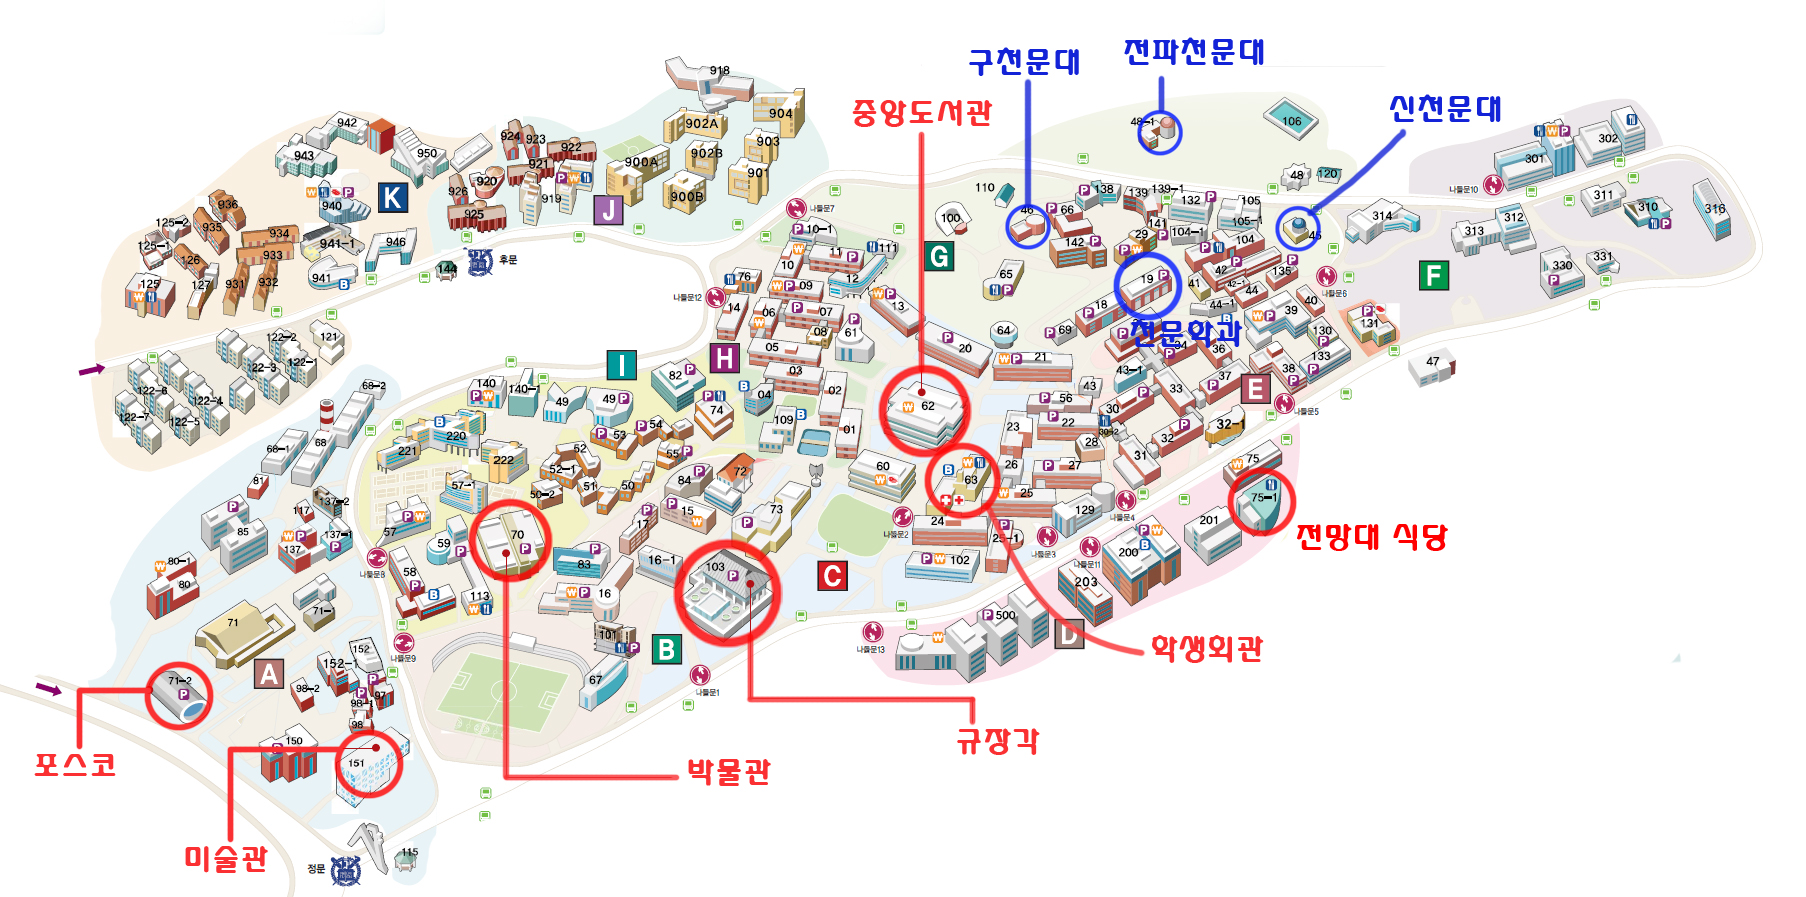
\includegraphics[width=0.95\textwidth]{./Figures/campus_map.jpg}
\legend{\textsf{캠퍼스 내 주요 건물}}
\end{center}
\end{figure}

\subsection{식당}
서울대학교는 신입생들이 (때로는 다닐 만큼 다닌 사람들도...) 가끔 길을 잃을 만큼
넓은 캠퍼스를 자랑한다.  그 넓이만큼 곳곳에 식당들도 많이 있다. 일단 다 먹고
살자고 하는 일이니 천문학과 대학원생들이 주로 이용하는, 혹은 이용가능한 식당에
대해 간단히 알아보자.\footnote{생활협동조합 직영 및 준직영 식당들의 메뉴 정보와
  운영시간 위치 등은 \url{http://www.snuco.com} 에서 자세히 확인할 수 있다.}
그외에 샤밥이라는 아이폰 어플과, inSNU라는 안드로이드 어플 등도 있으니
활용해보자.

\begin{description}
\item[\textsf{전망대(75-1동)}] \hfill \\
  천문학과 대학원생들의 주 이용 식당. 75-1동의 3, 4층에 위치하며 학생식당 중 19동에서 가장 가깝다. 보통 3층에 네 가지의 메뉴, 4층에 두세 가지의 메뉴가 제공된다.\\
  \hspace*{0.5cm}- 가격: 2500 / 3000 / 4000\\
  \hspace*{0.5cm}- 운영시간: 3층 - 11:00--14:00 / 4층 - 11:30--13:30, 17:00--19:00.\\
  \hspace*{0.5cm}- 주말은 토요일 점심만 4층이 운영되고 나머지는 휴관이다.\\

\item[\textsf{학생회관(63동)}] \hfill \\
  학생회관에 위치하는 식당으로 19동에서 갈 경우 식당으로 갈 때는 갈만하다는 생각이 들지만 올라올 때 많이 힘들다;; 학생회관인 만큼 주말까지 열려있으며 평일에는 저녁 9시까지 운영된다. 세 가지의 메뉴가 각각의 시간대별로 제공되며 지하에도 두 가지의 메뉴가 있다.\\
  \hspace*{0.5cm}- 가격 : 1700(B코너) / 2500 / 3000 \\
  \hspace*{0.5cm}- 운영시간 \hfill\\
  \hspace*{1cm} A코너 - 11:00--14:00, 16:30--18:30\\
  \hspace*{1cm} B코너 - 08:00--10:00, 11:00--14:00. 17:00--19:00\\
  \hspace*{1cm} C코너 - 10:00--16:30, 17:30--21:00\\
  \hspace*{1cm} 지하 - 11:00--13:00\\
  \hspace*{1cm} 주말 : 11:00--14:00, 17:00--19:00\\

\item[\textsf{공대간이식당(30-2동)}] \hfill \\
  전망대 만큼이나 가까이 위치한 식당이다. 짜장면, 짬뽕, 사천짜장이 고정 메뉴로 있으며 월~금 각각의 요일마다 정해진 덮밥 메뉴가 있다.\\
  \hspace*{0.5cm} - 가격 : 짜장면 2500원 / 짬뽕, 사천짜장, 덮밥류 3000원

\item[\textsf{솔밭식당(110동)}] \hfill \\
  거리상으로 상당히 가까우나 사실 잘 가게 되지는 않는 식당. 무려 학교보다도 더
  나이가 많은 식당이며 국수와 국밥류가 있다. 가끔 한 번씩 가기엔 나쁘지 않은
  식당.  2013년을 마지막으로 사라진다고 했는데... 아직은 열린 결말.

\item[\textsf{BBQ카페(32-1동 지하)}] \hfill \\
  치킨, 피자, 스파게티 등 여러 메뉴들이 있다. 학생식당들의 밥이 너무 먹기 싫은데
  밖에 나가기는 귀찮다거나 나갈 시간이 없을 때의 최선의 선택이다. 물론 치킨을
  좋아 할 경우에. 다른 외부업체들과 마찬가지로 학생할인이 된다.

\item[\textsf{반공연}] \hfill \\
  19동 뒷길로 올라가면 빠르게 갈 수 있는 식당으로 라면과 요일별로 정해진 밥이
  있다. 전망대 메뉴가 마음에 안들거나 라면이 급 땡길 때 가게 되는 식당이다.

\item[\textsf{기타}] \hfill \\
  이외에 서당골, 언덕방, 기숙사식당, 동원관식당 등의 학생식당이 있다. DOS TACOS,
  포베이, 비비고, 더키친, 파파이스 등의 외부업체들이 있다. 학교 탐방을 해 보고
  싶다거나, 다른 구역에 볼일이 있다거나 할 때 다른 식당들도 방문해보자.

\end{description}
\starbreak 밥만 먹고 살 수는 없다. 가끔 커피도 한 잔씩 마셔주고, 앉아서 이런 저런
이야기나 연구에 대한 토의도 할 수 있는 장소가 필요하다.
\begin{description}
\item[\textsf{The LAB(32-1동 1층)}] \hfill \\
  천문학과 대학원생들이 가장 많이 가는 곳이 아닐까 생각된다. 19동에서 전망대로
  가는 코스 중간에 위치하기 때문이다. 커피 등의 음료들과 간단한 간식거리들이
  있다.

\item[\textsf{Mug(공대신양)}] \hfill \\
  19동에서 아래로 내려가면 바로 만날 수 있는 공대신양에 위치한다. 연구에 지칠 때
  가끔 기분전환으로 갈 수 있는 곳이다. 손님(졸업한 선배 등)이 오면 자주 가는
  곳이기도 하다. 커피 등의 음료들과 샌드위치 등 간단한 음식들이 있다.

\item[\textsf{학생회관 스낵코너(63동)}] \hfill \\
  토스트 판매대, 토판이라고도 한다. 학생회관 1층 식당 옆에 위치하며 커피, 음료
  뿐만 아니라 샌드위치, 버거, 떡볶이와 순대까지 판매 한다. 위치가 위치이니 만큼
  항상 사람들로 붐빈다.

\item[\textsf{기타}] \hfill \\
  카페판코, 투썸플레이스, 파스쿠치 등의 카페들이 학교 곳곳에 위치한다.
\end{description}
\starbreak 간식거리를 살 수 있는 매점들 또한 곳곳에 위치하고 있다.
\begin{packed_item}
\item 일단 가장 접근성이 좋은 전망대 매점이 있다. 전망대 4층 입구쪽에 위치하고
  있으며 거리상으로 가장 가깝다기 보다는 보통 밥을 먹으러 가는 장소가 전망대이기
  때문에 가장 많이 이용되는 곳이다. 음료 및 과자 등 뿐만 아니라 간단한 문구류도
  구매할 수 있다.
\item 32-1동 지하(BBQ 옆)에 패밀리마트가 있다. 편의점이긴 한데 속지 말아야 할
  것은 11시가 되면 문을 닫는다.
\item 반공연 식당은 식당과 매점이 함께 운영되고 있다. 과자와 음료만 있다.
\item 중앙도서관 매점은 중앙도서관 터널, 뚜레쥬르와 같은 공간에 있으며 전망대
  매점과 마찬가지로 문구류 또한 구매할 수 있다. 편의점과 기숙사 매점을 제외하면
  학교내 매점 중 가장 오랜시간 열려있다. 밤 10시반까지 운영되며 시험기간엔
  연장운영이 된다.
\item 사회대 신양과 대학원 기숙사에는 각각 패밀리마트와 GS25가 있으며 이 두 곳은
  24시간 영업을 한다. 학부 기숙사(919동) 식당 옆의 매점은 새벽 두 시까지
  운영된다.
\end{packed_item}

\subsection{건물}
\begin{description}
\item[\textsf{학생회관(63동)}] \hfill \\
  학생들을 위한 시설들이 가장 많이 포함된 곳은 역시 학생회관이다. 매일 열려있는
  학생식당을 포함 보건소, 약국, 문구점, 서점, 은행 등 각종 시설들이
  있다. 천문학과 대학원생들은 학생회관을 갈 일이 실질적으로 별로 없긴 하지만
  학생회관에서 간단히 해결 할 수 있는 일들을 힘겹게 학교 밖으로 나가서 해결하는
  경우들이 간혹 있으니 학생회관에 어떤 것들이 있는지는 파악해 두는 것이 좋다.
\begin{packed_item}
\item 식당과 매점, 스낵코너
\item 보건소, 약국
\item 문구점, 서점
\item 농협, 신한은행
\item 복사/제본/인쇄
\end{packed_item}

\item[\textsf{중앙도서관}] \hfill
\begin{packed_item}
\item 중앙대출실은 도서관 4층에 위치하고있다(중앙도서관 터널은 3층!).
\item 평일 09:00$\sim$21:00 / 토요일 09:00$\sim$17:00 / 일요일 13:00$\sim$17:00
\item 대학원생의 경우 대출기간은 1개월이며 20권까지 대출이 가능하다.
\item 대출 연장은 2회까지 가능하다. 단, 주의할 점은 연장을 하면 한달이 추가가
  되는 것이 아니라 연장 순간부터 다시 한 달이 된다. 반납기한이 지나버리면 연장이
  불가능하며 다른 사람이 예약을 해 둔 경우에도 연장이 불가능하다.
\item 연체시 3일 이후부터 (이전 3일까지 소급하여) 1일/1권 당 100원의 연체료가
  발생한다. 연체료가 있을 경우 대여를 할 수 없으며, 연체료를 내지않으면 졸업도
  안시켜준다는 것 명심할 것.
\item 졸업시 유의할 점 : 졸업 시점에 대출 도서가 있으면 졸업 처리가 안된다. 잊지
  말자.
\item 간혹 빌린 책이 꼭 필요해서 반납 기한이 지난 것을 알면서도 '나중에 연체료
  내고 말지 뭐'라고 생각하고 반납을 안 하는 경우들이 있는데 이것은 양심을
  팔아먹는 일이다. 절대 해서는 안되는 행동이다.
\item 필요한 책이 있는데 비싸서 사기 힘들 경우 중앙 도서관에 구매 신청을
  하자. 연구팀에 따라서는 팀 예산으로 필요한 책을 자체 구매할 수 있기도 하다.
\item 영상자료실에서 영화를 볼 수 있는 시설도 있으며, 중앙대출실 로비에는 그 자리에서 읽을 수 있는 다양한 서적들과 심지어 만화책도 있다. (슬램덩크!)
\item 6개의 대형 열람실이 있다. 1$\sim$6층 중 4층을 제외한 각 층에 열람실이
  있으며 3층은 3A / 3B로 구분되어있다(입구는 동일).
\end{packed_item}
\starbreak 관악캠퍼스에는 중앙도서관 이외에
사회과학도서관/경영학도서관/국제학도서관/농학도서관/법학도서관이 있으며 찾는 서적
중 중앙도서관에 없는 책이 있는 경우도 있다(연구를 위해 찾는 책은 그런 경우가
없다고 봐도 무방하다;;;). 각 도서관의 대출 시간/방식에 맞춰 대출이 가능하다.

\item[\textsf{은행}] \hfill
  \begin{packed_item}
  \item 우체국 : 대학본부 측면
  \item 농협 : 39동/학생회관/자하연
  \item 신한은행 : 공대신양/학생회관
  \item 우리은행 : 500동/인문대신양
  \end{packed_item}
\item[\textsf{운동시설}] \hfill \\
  운동, 매우 중요하다. 중요성에 대한 설명은 더 하지 않겠다.
  \begin{packed_item}
  \item 공대 BK헬스장 : 19동에서 가장 가깝다. 비교적 작지만 거리에서 매우 큰
    이점이 있다.
  \item 포스코 : 헬스, 수영, 스쿼시 등을 할 수 있으며 정문 쪽에
    위치한다. 19동에서의 거리는 제법 멀지만 학교 오는 길에 운동을 하기엔 그리
    나쁘지 않다.
  \item 자연대 헬스장 : 500동 지하에 위치하며 사실상 천문학과 대학원생이 이용하엔
    힘든 위치이다.
  \item 더블에스 (대학원 기숙사 헬스장) : 대학원 기숙사에 위치하며 운영시간이
    길다는 장점이 있다. 기숙사에 사는 학생들에게 특히 좋다.
\end{packed_item}

\item[\textsf{행정업무}] \hfill \\
  행정업무를 가끔 직접 처리해야 할 경우가 있는데, 천문학과 대학원생이 갈 일이
  있는 곳은 315호를 제외하면 많지않다. 56동에 위치한 물리천문학부 행정실과
  대학본부. 500동의 자연대 행정실 등이다. 대략적인 위치가 어디인지는 파악해두자.
  성적표, 재학증명서 등의 서류는 2014년 현재 서울대학교 포털 사이트를 통해 신청
  및 발급받을 수 있다. 포탈을 확인하자.
\end{description}

\section{천문학과 행사 일정}
\subsection{졸업을 하기 위한 일정}
\begin{description}
\item[논문제출자격시험(논자시)] (3월 중순 / 9월 중순) 논자시를 통과하지 못하면
  졸업도 없다.
\item[학위논문제안발표(Proposal)] (3월 중순 -- 4월 초 사이 / 9월 중순 --10월 초)
  프로포절의 경우 해당 학기에 준비된 대학원생 모두가 하루에 발표한다.  프로포절을
  한 학기에 곧바로 학위논문을 발표할 수 없으니 졸업하려는 학기보다 한 학기 이전에
  프로포절을 하여야 한다.
\item[학위논문발표] (매학기 말) 졸업을 위한 최종 관문. 박사는 각자가 다른 시간에
  심사를 받고, 석사는 하루에 모두 심사받는다.
\end{description}

\subsection{천문학과 가족 행사}
천문학과 구성원들이 모두 참여하는 행사는 연초의 신년교례회, 봄(1학기)의 관악산
등반, 가을(2학기)의 MT가 있다.

\subsubsection{신년교례회 (1월 첫 주)}
매년 1월 초 천문학과의 구성원들이 모두 모이는 행사이다. 새로운 구성원(신임 교수,
대학원 신입생, 학부 진입생 등)을 소개하고 한 해를 되돌아보는 자리이며 또한
교수님들의 덕담으로 새로운 한 해를 열어나가는 행사이다.

신년교례회 이후에 대학원생들은 연구실 자리 추첨이 있다. 모든 대학원생이 참여하며
각자가 추첨을 통해 자기가 1년간 생활할 연구실 및 자리를
뽑는다. 석사/박사/신입생을 적절한 인원수로 나눈 후 추첨을 하며 신년교례회 당일
이사를 마치는 것을 원칙으로 한다. 모두의 원활한 이사와 활기찬 새해 시작을 위해
모두 참석하도록 하자.

\subsubsection{관악산 등반 / 바베큐 파티 (4월 중순--말)}
봄 관악산 등반은 매 1학기에 열리는 과 행사이다. 이런 전체 행사가 없다면 학교를 몇
년씩 다녀도 한 번도 가보지 못할 가능성이 농후한 관악산 등반의 기회를 제공한다. 산
타기가 죽기보다 싫다면 할 수 없지만 교수님들께서도 특별한 일정이 없으시다면
대부분 참여하시니 꼭 참여하자.  관악산이 근교에 있는 산 중에서는 비교적 험한
산이긴 하지만 올라가지 못 할 곳은 아니며 시간도 그리 오래 걸리지 않는다. 다만
어느 정도의 복장은 갖추자. 대충 입고 갔다가 간혹 등산객 아저씨에게 한 소리 듣기도
한다.

등반이 끝나면 바베큐 파티가 열린다. 특별한 사정이 생기지 않는다면 전파천문대에서
열리며 특히 신입생들에게는 천문학과 구성원들과 친해질 수 있는 좋은
기회이다. 신년교례회 때 간략하게 넘어간 새 구성원들을 소개하는 자리이기도 하다.

\subsubsection{천문학과 MT (10--11월)}
1학기에 관악산 등반이 있다면 2학기에는 천문학과 MT가 있다. 1박2일의 일정으로
떠나며 "관악산등반/바베큐파티" 보다 더 오랜 시간 구성원들과 친해질 수 있는 기회가
MT이다. 모두가 참여하는 레크리에이션도 있으며 교수님들의 새로운 모습도 볼 수 있는
즐거운 시간이다. 2학기(후기) 신입생들이 자신을 소개할 수 있는 행사이기도 하다.

\subsubsection{졸업축하연 (2월 / 8월 말, 졸업식 전)}
매 학기 졸업생들을 축하하기 위해 열리는 다과를 곁들인 간단한 행사이다. 졸업생들을
한자리에서 모두 축하해 줄 수 있는 자리이니 꼭 참여하자.

\subsubsection{각종 행사 사회}
신년교례회, 관악산 등반 후의 바베큐 파티, MT의 모두가 함께하는 시간에는 사회가
필요하다. 일반적으로 입학 1년 이내의 신입생이 사회를 보게 되며 신년교례회와
바베큐 파티는 1명, MT는 남/녀 두 명이 행사를 진행하게 된다.  보통 연속으로 사회를
시키는 경우는 잘 없지만, 너무 잘 할 경우 또 시킬지도 모른다. 기록이
3연속이었던가... 그래도 이왕이면 잘 하면 좋다. 칭찬 많이 해준다.

\section{콜로퀴움 및 공개행사}
\subsection{콜로퀴움}
콜로퀴움은 학기 중 매주 목요일 4시 15분에 학교 내/외부의 연사님을 초청하여 여는
세미나이다. 다양한 분야의 연구들의 현재 동향에 대해 알 수 있는 좋은 기회이며
자신이 잘 모르는 분야에 대한 식견을 넓일 수 있는 기회이기도 하다. 신입생들의 경우
관련 분야가 아니거나 혹 관련 분야라 하더라도 구체적인 내용이 많이 이해를 잘
못하여 참석을 꺼리는 경우가 있는데 이는 대부분의 대학원생 모두가
마찬가지이다. 완전히 이해하지 못하더라도 다양한 분야의 내용을 들어두면 도움이 될
날이 있으니 꼭 참여하도록 하자.

콜로퀴움이 끝나면 간단한 다과가 열린다. 콜로퀴움 다과는 학생들과 연사님 간의
질문을 위한 시간으로 박사 학위 소지자들의 출입이 원칙적으로는 금지되어있다. 약 한
시간의 강연이 끝난 후 5시 15분 즈음에 304호에서 가진다. 보통 3~40분의 시간이
주어지며 콜로퀴움 당시 교수님들의 눈치가 보여 하지 못했던 매우 기초적인
질문이라도 부담 없이 할 수 있는 자리이다. 가끔 일정 변경으로 다른 요일, 혹은 다른
시간에 열리기도 한다. 그리고 수업에서 초정연사의 강의가 공개적으로 열릴 때가
있다. 이 경우 행정실에서 메일을 보내주고, 게시판에도 공지가 되니 항상 확인을
하자.

\subsubsection{콜로퀴움 도우미}
매 콜로퀴움마다 두 명씩 콜로퀴움 도우미를 해야 한다. 한 사람이 한 학기에 한 번을
하게 된다. 보통 도우미를 해 본 경험이 있는 선배와 신입생을 같이 배정해주므로
걱정하지 말고 콜로퀴움 전날에 선배를 찾아가자. 콜로퀴움 도우미가 해야 할 일은
크게 두 가지로 세미나 준비와 다과 준비이다.

세미나 준비는 연사의 발표를 위한 사전 준비이다. 연사님의 노트북으로 바로 발표를
하는 경우도 있지만 일단 행정실에서 노트북 및 레이저 포인터를 빌려 준비를 해
두어야 한다.

콜로퀴움 후에 열릴 다과 또한 준비해야 한다. 행정실에서 미리 카드를 받아두어야하며
보통 서울대입구 또는 낙성대에 위치한 GS슈퍼마켓을 이용한다(배달을 해 주기 때문에
상당히 편리하다). 제한된 금액으로 과일/과자/음료수 등을 준비해야 하므로 도우미의
센스를 엿볼 수 있는 부분이다. 가끔 구성이 학생들 마음에 들지 않을 경우 주변
대학원생들에게 까이기도 한다... 보통 오전 중에 미리 구입을 해 적당한 시간에
배달을 받는다. 콜로퀴움이 끝나고 바로 다과가 시작되기 때문에 콜로퀴움이 시작되기
전 적당한 준비를 마무리 해 두어야 한다. 그리고 발표가 끝난 후 질의응답 시간에
조금 미리 나와서 준비를 완료하면 된다. 간혹 다과 준비에 심취해서 노트북 준비와
세미나실 세팅(매우 중요!!)을 잊어버리는 경우가 있는데, 연사님에게 큰 실례가
되므로 주의하자. 또한 다과가 끝난 후 세미나실 정리와 다과 마무리 청소도 도우미가
해야 할 역할이다.

\subsection{공개행사}
1998년부터 1년에 6회씩 여는 행사이다. 일반인들을 대상으로 하여 천문학 강연 및
실험, 관측 시설 견학을 한다. 날이 좋은 경우 망원경을 이용한 별보기 행사를
진행한다. 이를 통해 일반인이게 학과를 소개하고 우리가 연구하는 것을 알리며
천문학에 대한 관심을 높이기 위한 취지이다. 공개행사는 과의 중요한 행사 중
하나로, 대학원생들과 학부생 그리고 교수님의 참여로 이루어진다. 총 6회 중 한 회에
박사 2-3명, 석사 3-4명 정도가 도우미로 참여한다. 도우미들 중 한두 명이 일반
대중을 위한 강연을 하고, 관련 프로그램에 따른 실험 또는 실습을 진행하며 이후에
참여한 일반인들을 인솔하고 진행을 돕는다. 날이 좋은 경우 망원경을 설치하여
천체들을 보여주고, 구천문대나 신천문대의 시설 등을 이용하여 천체 관측을 도와주는
것이 기본적으로 포함된다.


\section{행정실 장비 관리}
천문학과 행정실에서는 쾌적한 토의 및 연구 활동을 위해 다양한 전산 장비들을
구비하고 있다. 이 물품들은 공공 물품이므로, 이를 사용하기 위해서는 지켜야할
우리만의 아름다운 합의 사항이 있다. 이들에 대해 알아보자.

가용한 전산 장비 목록은 다음과 같다.
\begin{packed_item}
\item 노트북 4개
\item 프로젝터 3개
\item 레이저 포인터 9개
\end{packed_item}

\subsection{전산 장비 빌리기}
행정실에서 전산장비를 빌리는 건 전혀 어렵지 않다. 전산장비를 대여함에 있어서
확실히 해야 할 일은 딱 한 가지뿐이다. 바로 대여 장부를 성실하게 작성하는
일. 행정실에 들어가서 장비를 대여해 나오는 모든 일을 순서대로
진행해보자. 행정실에 들어가 입구를 등지고 섰을 때, 오른쪽에 있는 캐비넷에
전산장비 일체가 보관되어있다. 그리고 그 왼쪽 선반(조교님 책상 옆)에 대여 장부가
놓여있다. 먼저 원하는 전산 장비를 캐비넷에서 찾는다. 전산장비의 가방(케이스)을
보면 그 장비의 번호가 붙어있을 것이다. 설명하는 것이 귀찮을 정도로 간단한
작업이다. 이제 대여 장부를 열어보자. 대여 장부는 표 형식으로 간단하게 되어있어
누구나 그냥 보면 작성할 수 있다. '장비를 빌려간 날짜와 시간, 빌려간 사람,
지도교수, 대여자의 연락처, (방금 확인한) 빌려간 장비번호'를 기입하도록
되어있다. 여기까지 다 작성했는데도 옆에 칸이 남을 것이다. 마지막 칸은 장비를
되돌려 놓은 날짜와 시간을 기록하는 칸이다. 즉, 잘 쓰고 얌전히 제자리에 돌려놓은
후 마저 작성하면 된다. 성실하게 기입하였다면 이제 행정실을 나가도 좋을
것이다. 하지만 마지막으로 한 가지 더 확실히 해야 할 것이 있다. 장비를 제자리에
돌려놓았는지 하는 것이다. 간혹 여러 장비를 한꺼번에 빌려 쓰고는 전원선이며 레이저
포인트들을 아무 가방에나 제짝이 아닌 것끼리 모아놓는 경우가 있다. 이럴 경우
뒷사람이 매우 불편하고, 귀찮게 되므로 {\textbf{\emph{제발 제자리에 돌려놓도록
      하자.}}}

\subsection{행정실의 사진 장비}
천문학 및 천문학 실험 등의 수업에서 일주운동관측과 같은 과제가 나올 시 행정실에서
별 사진을 찍을 수 있는 장비들을 빌릴 수 있다. 사용 가능한 사진 장비는 카메라,
릴리즈, 삼각대 등이 있다. 이 때 중요한 것은 장비들이 대개 고가이기 때문에 장비를
빌릴 때 담당과목의 조교와 함께 가서 빌려야 한다. 각 사진장비 역시 기기마다 번호가
붙어있으며 담당조교는 이를 확인하고 대여 장부를 작성하여야한다. 대여 장부에는
'대여일시, 지도교수(수업명), 대여자 (+ 조교) 성명과 연락처, 빌려간 장비내역,
반납일시'를 작성하도록 되어있다. 장비를 반납할 때는 대여할 때와 마찬가지로 조교가
반드시 동행해야하고 반납 전에 장비의 이상 유무를 확인해야한다.

\subsection{천문대 이용}
관측 수업이나, 기타 목적을 이용한 천문대 이용도 가능하다. 서울대 안에 있는
구천문대와 신천문대의 경우 천문대 열쇠 대여 장부를 작성한 뒤 열쇠 (구천문대),
카드키 (신천문대)를 빌려 출입할 수 있다. 신천문대 사용시에는 신천문대
상주자들에게 미리 연락을 해 두자.

\subsection{복사기 / 프린터 / 플로터 / 스캐너 위치}
\begin{packed_item}
\item 복사기 : 행정실
\item 프린터 : 315A 호 (행정실 옆방) 행정실과 연결되어있지만 출입은 315A 문으로
  하자. 컬러/흑백 레이저 프린터가 각각 있으며 네트워크로 연결되어있으니 각자의
  연구실에서 출력 후 프린트 물을 찾아가면 된다. 간혹 프린트를 해 두고 잊어버려
  장시간 방치되는 경우가 있는데 그런 일이 없도록 바로바로 찾아가도록
  하자. 일과시간이 끝난 후에는 이용 후 반드시 불을 끄고 문을 잠가야 한다.
\item 스캐너 : 308B 호 (전산실)
\item 플로터 : 서버실에 있고, 학회 참가 시 출력할 포스터를 뽑을 때 주로
  사용한다. 2013년 업그레이드 되어 종이가 아닌 천에 포스터를 뽑을 수 있게
  되어있다!
\end{packed_item}

\section{소모임 소개}
\subsection{얌(YAM)}
Young Astronomers Meeting(YAM)은 젊은 천문 우주과학자들의 모임으로써, 2005년
4월에 재결성 된 학술 교류 및 친목을 도모하기 위한 모임이다. 천문학회 정기
학술대회의 Night session에 얌 모임이 있으며, 방학 때마다 정기모임을 통하여 국내
대학원생들 및 박사 후 연구원들의 친목을 다지고, 나아가 East Asia Young
Astronomers Meeting(EAYAM), Korea-Japan Young Astronomers Meeting(KJYAM) 등을
직접 개최하여 동아시아 혹은 한일 젊은 천문우주과학자들 사이의 학술 교류 및 친목을
도모하고 있다. 자유로운 YAM 분위기에서는 토론과 대화를 통해 자기 분야가 아닌 타
연구 분야를 쉽게 배울 수 있고, 단기적으로는 대학원생들의 견문을 넓힐 수 있고,
장기적으로는 새로운 공동연구관계를 만들 수 있다.

\subsection{저널클럽}
저널클럽(Journal Club)은 다양한 연구 분야에 대한 지식을 넓히고 토론능력을
향상시키기 위하여 학과 내 대학원생들이 자발적으로 참여하고 운영하는
모임이다. 학기 중의 정기모임은 격주로 열리며 방학 중에는 매주 모임을
가진다. 저널클럽 모임에서는 각 대학원생의 연구내용을 공유하고 토론할 수 있는
시간을 갖거나, 특정분야의 논문들을 선정하여 매주 한편씩 읽고 토론함으로써 그
분야에 대한 심층적인 지식을 넓히기도 하고, arXiv등을 활요해서 최신 연구 동향에
대한 관심사를 공유하기도 하는 등 다양한 시도를 통해 목적 성취를 위해 노력하고
있다. 초기에는 우리 은하 및 외부 은하 연구에 관련된 주제를 주로 다루는 모임으로
출발하였으나, 현재는 다양한 분야의 학생들이 다양한 주제에 관해 서로의 관심사와
지식을 공유하고 있다. 저널클럽에서는 학생들의 자유로운 모임이므로 서로 궁금한
부분에 대하여 부담 없이 질문하고 토론할 수 있다..

2014년 초 현재에는 SNS 페이스북 그룹페이지를 통해 모임을 준비하고 있다.
\begin{packed_item}
\item 학과 홈페이지 저널클럽란
  \href{http://astro1.snu.ac.kr/home/kor/Journal/Journal_info.asp?globalmenu=6&localmenu=2}{바로가기}
\item 저널클럽 토론 게시판: \url{http://astro.snu.ac.kr/jc}
\item 저널클럽 페이스북 그룹 :
  \url{https://www.facebook.com/groups/snu.astrojc/}
\end{packed_item}

\section{소통하기}
\subsection{교수님과 소통하기}
대학원생이 자신의 지도교수님과 소통하는 방식은 크게 3가지로 나눌 수
있다. 팀미팅, 개인 면담, 그리고 수시로 주고받는 이메일을 통해서이다.

먼저 팀 미팅은 팀마다 분위기가 다르기에 간단히만 설명하자면, 정기적으로(일주일에
두 번 하는 팀도 있고 한 달에 한번 하는 팀도 있다.) 모여서 팀원들이 돌아가며
자신이 그 동안 한 일에 대해 발표하고 교수님/팀원들과 토론하는 방식으로 진행되고,
자기 연구와 관련된 논문을 리뷰하기도 한다. 하나 상기할 점은, 교수님과 일대일로
대화하는 시간이 아니라 팀원 전체에게 발표하는 시간이라는 점이다. 더 이상의 자세한
설명은 생략하니 자기 팀의 팀 미팅 분위기는 몸으로 깨우치길 바란다.

개인 면담의 경우 시간을 정확히 정해 두는 교수님도 있는 반면 학생들에게 딱히
요구하지 않으시는 교수님도 있다. 교수님과 일대일로 토론을 하기에 보통 팀 미팅 때
했던 얘기보다 더 심도 깊은 토론을 하게 되고, 한참 연구가 진행 중일 때는 뭔가 잔뜩
준비해서 들고 갔더니 준비한 것들에서 오류가 있어서 수정해야 할 것들을 훨씬 많이
짊어지고 자리로 비틀비틀 돌아오는 일도 흔하다. 그만큼 연구 진척에는 정말 도움이
되지만, 정신적 데미지를 최소화하려면 팀 미팅보다도 더 철저한 준비가
요구된다. 아직 맡은 연구가 없는 신입생들은 따로 안 부르실 지도 모르지만, 그래도
학기 시작하면 '연구하고 싶어요' 라고 얼굴에 써붙이고 한번쯤은 찾아가
보자. 찾아오는 학생 내치는 교수님은 없다. 오히려 선생님이 시간적으로 여유가
있으신 상황이라면 준비가 덜 되었더라도 수시로 찾아가 보자. 토의 끝에 지지부진한
연구 진척 상황에 힌트를 얻고 오는 일도 많다. 무엇보다 중요한 점은
\textbf{면담시간 까먹지 말자}! 피본다.

e-mail은 지도교수님 뿐만 아니라 다른 협동 연구자들과도 가장 많이 소통하게 되는
매체이다. 용건만 간단히 적어도 되지만 몇 가지 팁을 주자면.
\begin{packed_item}
\item 모르는 사람 (ex:지도교수 배정 전에 문의 메일을 보내는 경우)에게 보낼 때는
  일단 자기가 누구인지 밝히자. 기본이다. 그리고 이럴 땐 조금 딱딱하더라도 편지
  형식을 갖춰 보내는 것이 좋다.
\item 연구에 관련된 오고가는 메일: 설마 계속 Re:Re:달린 메일에 저는 누구누구
  입니다 부터 적지는 않겠지? 용건만 간단히 적으면 되겠다.
\item 새로운 메일로 쓰기보다, 답장으로 보내 이전 교신 기록들이 아래에 뜨도록 하는
  편이 양쪽 모두에게 편하다.
\item 연구를 같이 진행 중인 선배나 다른 협동 연구자가 있으면 참조(C.C)로 다 같이
  볼 수 있게 보내자.
\item 답장은 가급적 빨리 하자 대답하는데 오래 걸릴 사안이면 ‘확인했습니다.’
  ‘해보겠습니다.’ 정도로라도 보내자. 수신확인 기능은 네이버, 다음 같은 국내
  포털사이트 메일에만 있다. 아! 물론 XXX께,YYY 드림 정도는 잊지말고 쓰자.
\end{packed_item}
교수님과 휴대폰으로 통화하는 경우는 드물다. 전화 예절까지 알려줄 필요는 없다고
생각하여 생략한다. 알아서 잘...

지도교수님과의 원활한 관계 유지는 대학원 생활에서 자신의 연구만큼이나 중요한
부분이다. 다행히 우리 과 교수님들은 대게 인자하시지만, 교수님들도 사람이니만큼
학생이 계속 미운 짓을 했다간 언제 어떻게 관계가 틀어질지 모른다. 한번 교수님과
관계가 틀어지면 그 후의 대학원 생활은 헬게이트 오픈이니 그렇게 되기 전에 알아서
잘하자.

\subsection{대학원 동료들과 소통하기}
대학원 동료들과 연구실 사람들이 밥 먹으러 갈 때 따라가자! 아는 사람 없는 뻘쭘한
학기 초에 연구실 사람들과 친해지는 최고의 방법이다. 학기 초에 전체 주소록이 담긴
pdf파일이 astro 메일로 올 테니 바탕화면 한구석에 놓고 누군가에게 연락할 일이 있을
때 활용하면 좋다. \texttt{master@astro.snu.ac.kr, phd@astro.snu.ac.kr,
postdoc@astro.snu.ac.kr, prof@astro.snu.ac.kr}을 통해 전체 메일을 보낼 수
있다. 순서대로 석사과정, 박사과정, 포스닥들, 교수님들. 자기가 어떤 모임을
주도하게 되었다던가, 엠티책이 되었다던가 해서 공지사항을 돌릴 일이 있으면
활용하자. 모두에게 가는 만큼 전체메일을 쓸 때는 신중하게 보내자. ‘주말인데 술 한
잔 하실 분’ 같은 내용을 전체메일로 뿌렸다간 산더미 같은 일에 짓눌려 늦게까지 퇴근
못하고 있던 선배의 분노를 정면으로 받게 될지도 모른다.

\section{연구실 에티켓}
\subsection{연구실 에티켓}
\begin{packed_item}
\item 잡담은 적당히...
\item 전화는 나가서 받자!
\item 음악은 헤드폰으로 음량을 주의하여 듣자!
\item 마지막으로 나가는 사람은 문단속, 전열기 및 전등 끄기
\item 연구실 내에서 양치하지 말자!
\item 지나친 애정행각은 주위 사람들의 연구에 방해가 될 수 있음!
\item 주기적인 대청소를 하고, 청소에 적극 참여하자.
\item 자기 자리는 개인 공간이기도 하지만 공동 연구실의 일부이기도 하니 쓰레기
  등을 방치하지 말고 치우자.
\item 악기 연주는 집에서.
\item 냄새 나는 음식을 연구실에서 먹지 말자.
\item 연구실에서 각자 키우는 화분들은 책임지고 관리하자.
\item 흡연은 정해진 곳에서, 꽁초는 쓰레기통에!
\item 연구실에서 개인 활동으로 인한 소리는 적당히... (웃긴 동영상 혼자 보면서
  킄킄 대지 말고 같이 보자...)
\end{packed_item}

\subsection{공공장소 에티켓}
\subsubsection{휴게실}
\begin{packed_item}
\item 식기 사용 후에는 설거지를 해놓자!
\item 냉장고 문이 닫혔는지 확인!
\item 냉장고 안 다른 사람의 음식을 탐내지 말자!
\item 냉장고 안에 자신이 넣은 음식은 자신이 처리하자!
\item 냉장고 안 얼음을 다 쓴 사람이 물을 다시 얼려 놓자!
\item 휴게실 사용 후 뒷정리 (냄새나는 음식 먹은 뒤 환기)!
\item 복도에서 실내화 질질 끌고 다니지 않기!
\item 나올 때 불/에어컨(히터) 끄기
\end{packed_item}

\subsubsection{프린터실}
\begin{packed_item}
\item 자기가 프린트 한 것 바로바로 찾아가기
\item 일과시간 이후 나올 때 꼭 불 끄고 문 잠그기
\item 색이 꼭 필요하지 않은 경우 흑백 프린터를 사용하자.
\item 개인적인 인쇄물 출력은 자제하자
\item 양면 인쇄를 적극 활용하여 이면지 양산을 줄이자.
\end{packed_item}


